% 文档类型
\documentclass[a4paper]{article}

% 引用包裹
\usepackage{geometry}
\usepackage{bm}
\usepackage{cmap}
\usepackage{ctex}
\usepackage{cite}
\usepackage{color}
\usepackage{float}
\usepackage{xeCJK}
\usepackage{amsthm}
\usepackage{amsmath}
\usepackage{amssymb}
\usepackage{setspace}
\usepackage{geometry}
\usepackage{hyperref}
\usepackage{enumerate}
\usepackage{indentfirst}
\usepackage{graphicx}
\usepackage{caption, subcaption}
\usepackage[cache=false]{minted}

\geometry{left=2.0cm, right=2.0cm, top=1.5cm, bottom=1.5cm}
\newcommand{\matlabcode}[1]{
	\inputminted[mathescape,tabsize=2]
	{matlab}{../#1}
}
\begin{document}

\section{计算实习题 P50 第2题}
\subsection{解题方案}
	代码如下,将主程序中n的值修改为10和20来计算不同的情况
\subsection{图片}
	\begin{figure}[ht]
		\begin{subfigure}[t]{0.5\textwidth}
		\centering
		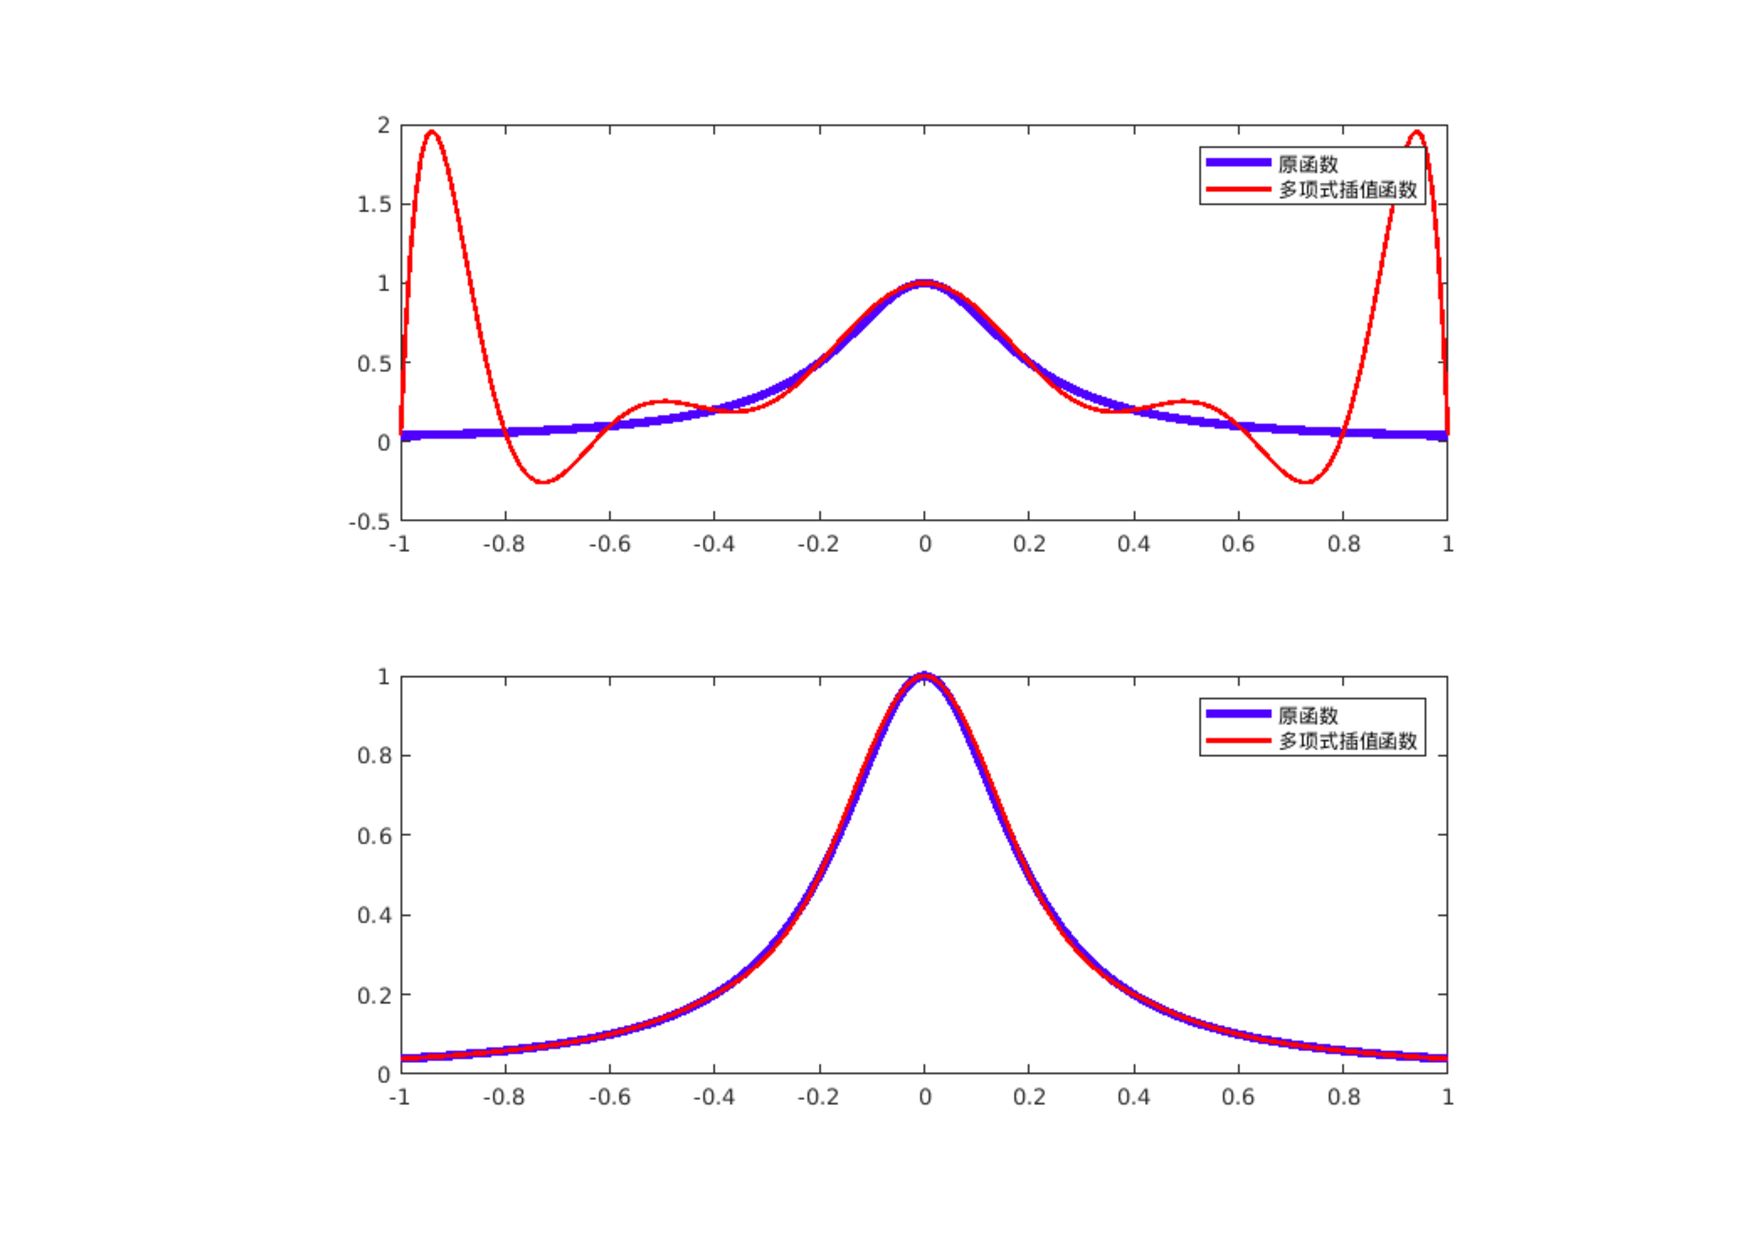
\includegraphics[width=1.2\textwidth]{figure/n10bmp.pdf}
		\subcaption*{n=10}
		\end{subfigure}
		\quad
		\begin{subfigure}[t]{0.5\textwidth}
		\centering
		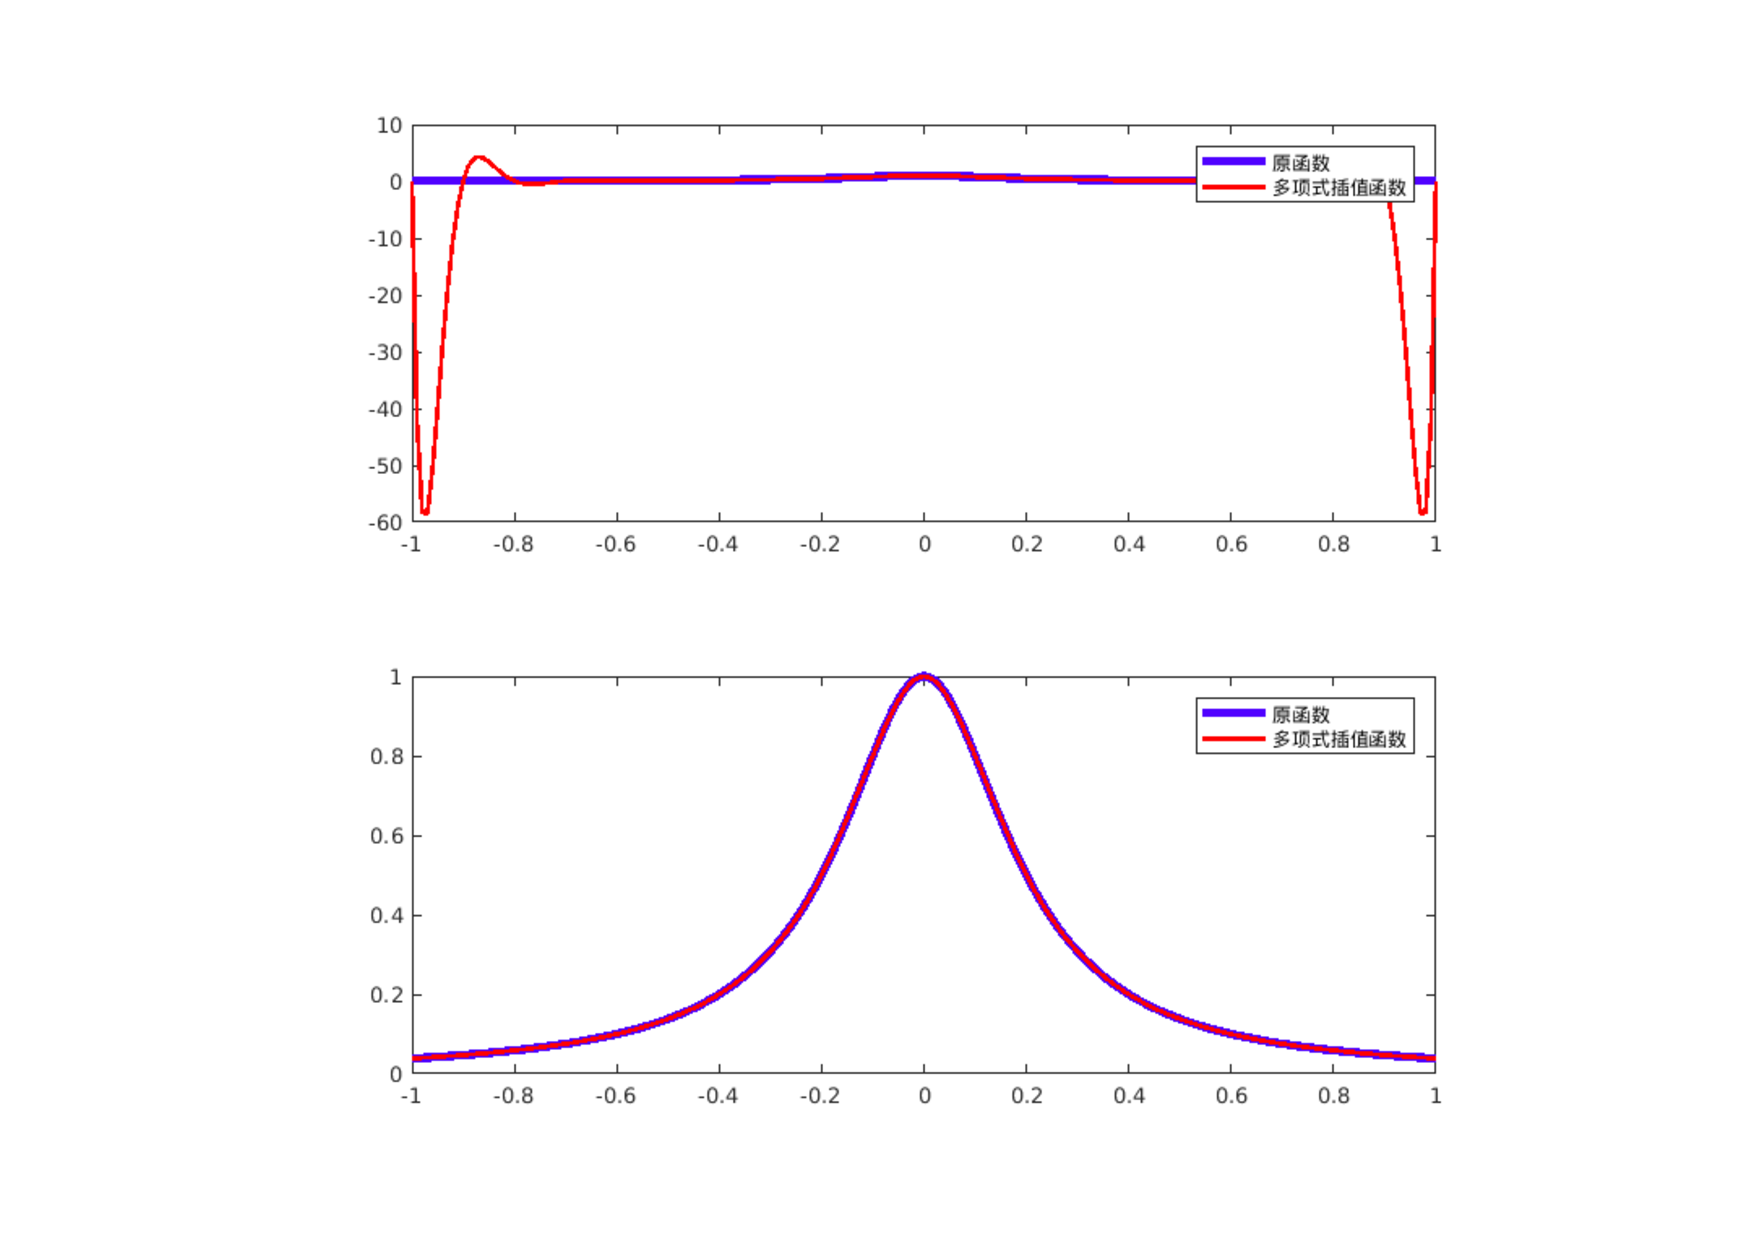
\includegraphics[width=1.2\textwidth]{figure/n20bmp.pdf}
		\subcaption*{n=20}
		\end{subfigure}
	\end{figure}
\subsection{代码}
\subsubsection{主程序}
	\matlabcode{task1.m}
\subsubsection{多项式插值}
	\matlabcode{poly_interpolation.m}
\subsubsection{三次样条插值}
	\matlabcode{spline_interpolation.m}

\section{补充练习}
\subsection{代码}
\subsubsection{主程序}
	\matlabcode{main.m}
\subsubsection{三次样条插值}
	同上一题的代码。写完第一题的代码后,在其基础上改得第二题代码,但是没有保留原始版本,只好共用了一份代码。
\subsection{插值图像}
	\begin{figure}[ht]
		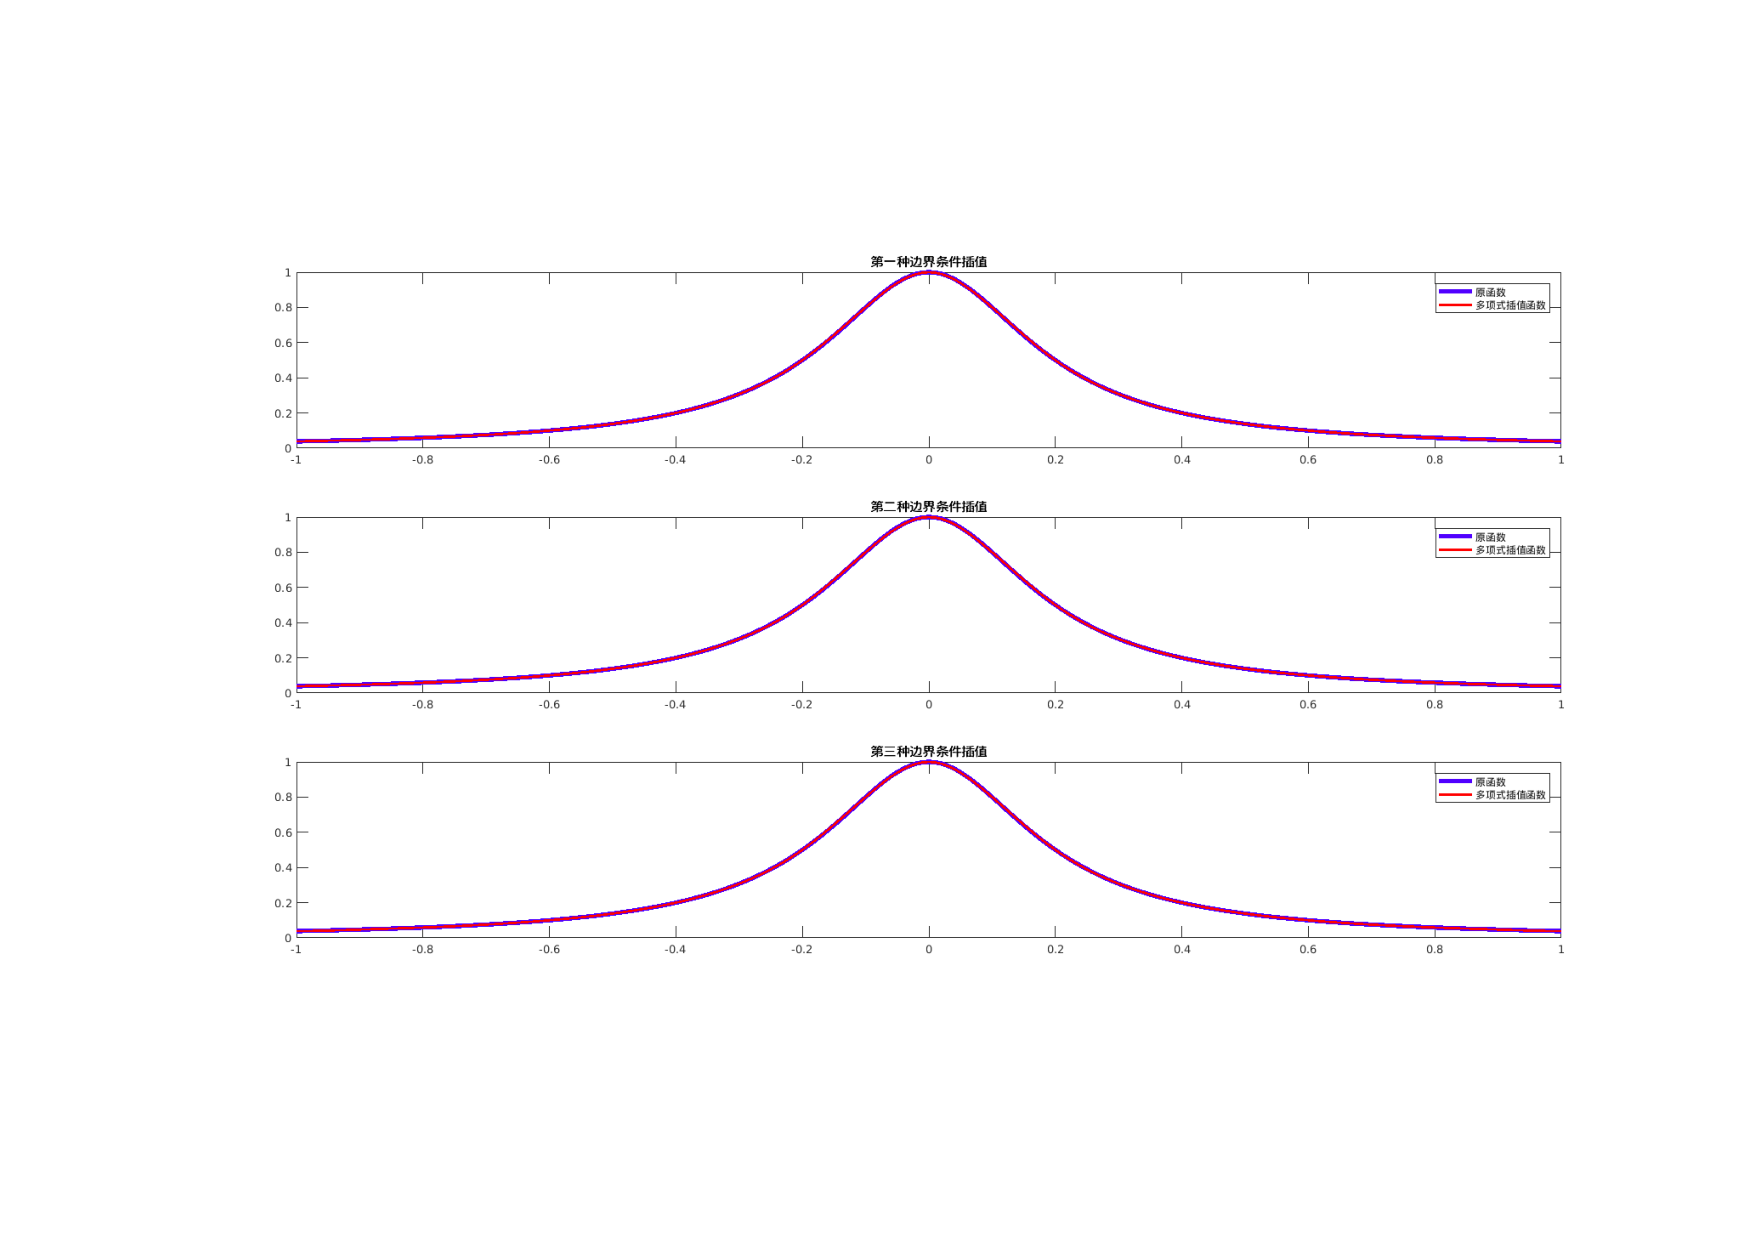
\includegraphics[width=1\textwidth]{figure/addtionpng.pdf}
	\end{figure}
\end{document}

  